% Options for packages loaded elsewhere
\PassOptionsToPackage{unicode}{hyperref}
\PassOptionsToPackage{hyphens}{url}
\PassOptionsToPackage{dvipsnames,svgnames,x11names}{xcolor}
%
\documentclass[
  12pt,
]{book}
\usepackage{amsmath,amssymb}
\usepackage{lmodern}
\usepackage{iftex}
\ifPDFTeX
  \usepackage[T1]{fontenc}
  \usepackage[utf8]{inputenc}
  \usepackage{textcomp} % provide euro and other symbols
\else % if luatex or xetex
  \usepackage{unicode-math}
  \defaultfontfeatures{Scale=MatchLowercase}
  \defaultfontfeatures[\rmfamily]{Ligatures=TeX,Scale=1}
\fi
% Use upquote if available, for straight quotes in verbatim environments
\IfFileExists{upquote.sty}{\usepackage{upquote}}{}
\IfFileExists{microtype.sty}{% use microtype if available
  \usepackage[]{microtype}
  \UseMicrotypeSet[protrusion]{basicmath} % disable protrusion for tt fonts
}{}
\makeatletter
\@ifundefined{KOMAClassName}{% if non-KOMA class
  \IfFileExists{parskip.sty}{%
    \usepackage{parskip}
  }{% else
    \setlength{\parindent}{0pt}
    \setlength{\parskip}{6pt plus 2pt minus 1pt}}
}{% if KOMA class
  \KOMAoptions{parskip=half}}
\makeatother
\usepackage{xcolor}
\usepackage{color}
\usepackage{fancyvrb}
\newcommand{\VerbBar}{|}
\newcommand{\VERB}{\Verb[commandchars=\\\{\}]}
\DefineVerbatimEnvironment{Highlighting}{Verbatim}{commandchars=\\\{\}}
% Add ',fontsize=\small' for more characters per line
\usepackage{framed}
\definecolor{shadecolor}{RGB}{248,248,248}
\newenvironment{Shaded}{\begin{snugshade}}{\end{snugshade}}
\newcommand{\AlertTok}[1]{\textcolor[rgb]{0.94,0.16,0.16}{#1}}
\newcommand{\AnnotationTok}[1]{\textcolor[rgb]{0.56,0.35,0.01}{\textbf{\textit{#1}}}}
\newcommand{\AttributeTok}[1]{\textcolor[rgb]{0.77,0.63,0.00}{#1}}
\newcommand{\BaseNTok}[1]{\textcolor[rgb]{0.00,0.00,0.81}{#1}}
\newcommand{\BuiltInTok}[1]{#1}
\newcommand{\CharTok}[1]{\textcolor[rgb]{0.31,0.60,0.02}{#1}}
\newcommand{\CommentTok}[1]{\textcolor[rgb]{0.56,0.35,0.01}{\textit{#1}}}
\newcommand{\CommentVarTok}[1]{\textcolor[rgb]{0.56,0.35,0.01}{\textbf{\textit{#1}}}}
\newcommand{\ConstantTok}[1]{\textcolor[rgb]{0.00,0.00,0.00}{#1}}
\newcommand{\ControlFlowTok}[1]{\textcolor[rgb]{0.13,0.29,0.53}{\textbf{#1}}}
\newcommand{\DataTypeTok}[1]{\textcolor[rgb]{0.13,0.29,0.53}{#1}}
\newcommand{\DecValTok}[1]{\textcolor[rgb]{0.00,0.00,0.81}{#1}}
\newcommand{\DocumentationTok}[1]{\textcolor[rgb]{0.56,0.35,0.01}{\textbf{\textit{#1}}}}
\newcommand{\ErrorTok}[1]{\textcolor[rgb]{0.64,0.00,0.00}{\textbf{#1}}}
\newcommand{\ExtensionTok}[1]{#1}
\newcommand{\FloatTok}[1]{\textcolor[rgb]{0.00,0.00,0.81}{#1}}
\newcommand{\FunctionTok}[1]{\textcolor[rgb]{0.00,0.00,0.00}{#1}}
\newcommand{\ImportTok}[1]{#1}
\newcommand{\InformationTok}[1]{\textcolor[rgb]{0.56,0.35,0.01}{\textbf{\textit{#1}}}}
\newcommand{\KeywordTok}[1]{\textcolor[rgb]{0.13,0.29,0.53}{\textbf{#1}}}
\newcommand{\NormalTok}[1]{#1}
\newcommand{\OperatorTok}[1]{\textcolor[rgb]{0.81,0.36,0.00}{\textbf{#1}}}
\newcommand{\OtherTok}[1]{\textcolor[rgb]{0.56,0.35,0.01}{#1}}
\newcommand{\PreprocessorTok}[1]{\textcolor[rgb]{0.56,0.35,0.01}{\textit{#1}}}
\newcommand{\RegionMarkerTok}[1]{#1}
\newcommand{\SpecialCharTok}[1]{\textcolor[rgb]{0.00,0.00,0.00}{#1}}
\newcommand{\SpecialStringTok}[1]{\textcolor[rgb]{0.31,0.60,0.02}{#1}}
\newcommand{\StringTok}[1]{\textcolor[rgb]{0.31,0.60,0.02}{#1}}
\newcommand{\VariableTok}[1]{\textcolor[rgb]{0.00,0.00,0.00}{#1}}
\newcommand{\VerbatimStringTok}[1]{\textcolor[rgb]{0.31,0.60,0.02}{#1}}
\newcommand{\WarningTok}[1]{\textcolor[rgb]{0.56,0.35,0.01}{\textbf{\textit{#1}}}}
\usepackage{longtable,booktabs,array}
\usepackage{calc} % for calculating minipage widths
% Correct order of tables after \paragraph or \subparagraph
\usepackage{etoolbox}
\makeatletter
\patchcmd\longtable{\par}{\if@noskipsec\mbox{}\fi\par}{}{}
\makeatother
% Allow footnotes in longtable head/foot
\IfFileExists{footnotehyper.sty}{\usepackage{footnotehyper}}{\usepackage{footnote}}
\makesavenoteenv{longtable}
\usepackage{graphicx}
\makeatletter
\def\maxwidth{\ifdim\Gin@nat@width>\linewidth\linewidth\else\Gin@nat@width\fi}
\def\maxheight{\ifdim\Gin@nat@height>\textheight\textheight\else\Gin@nat@height\fi}
\makeatother
% Scale images if necessary, so that they will not overflow the page
% margins by default, and it is still possible to overwrite the defaults
% using explicit options in \includegraphics[width, height, ...]{}
\setkeys{Gin}{width=\maxwidth,height=\maxheight,keepaspectratio}
% Set default figure placement to htbp
\makeatletter
\def\fps@figure{htbp}
\makeatother
\setlength{\emergencystretch}{3em} % prevent overfull lines
\providecommand{\tightlist}{%
  \setlength{\itemsep}{0pt}\setlength{\parskip}{0pt}}
\setcounter{secnumdepth}{5}
\usepackage{booktabs}
\usepackage{color}
\usepackage{tcolorbox}
\usepackage{float}
\graphicspath{ {images/} }

\newenvironment{rmdremind}
  {\begin{tcolorbox}[width=\textwidth, 
                     colback = {white}, 
                     title = {\textbf{Remember}}, 
                     colbacktitle = lightgray,
                     coltitle = black]
  \begin{includegraphics}[scale = 1]{remind.png}
  \begin{itemize}}
  {\end{itemize}
  \end{includegraphics}
  \end{tcolorbox}}

\newenvironment{rmdnote}
  {\begin{tcolorbox}[width=\textwidth, 
                     colback = {white}, 
                     title = {\textbf{Note}}, 
                     colbacktitle = lightgray,
                     coltitle = black]
  \begin{includegraphics}[scale = 1]{pencil.png}}
  {\end{includegraphics}
  \end{tcolorbox}}
  
\newenvironment{rmdexercise}
  {\begin{tcolorbox}[width=\textwidth, 
                     colback = {white}, 
                     title = {\textbf{Exercise}}, 
                     colbacktitle = lightgray,
                     coltitle = black]
  \begin{includegraphics}[scale = 1]{exercise.png}}
  {\end{includegraphics}
  \end{tcolorbox}}
  
\newenvironment{rmdinfo}
  {\begin{tcolorbox}[width=\textwidth, 
                     colback = {white}, 
                     title = {\textbf{Info}}, 
                     colbacktitle = lightgray,
                     coltitle = black]
  \begin{includegraphics}[scale = 1]{info.png}}
  {\end{includegraphics}
  \end{tcolorbox}}  
  
\newenvironment{rmdwarning}
  {\begin{tcolorbox}[width=\textwidth, 
                     colback = {white}, 
                     title = {\textbf{Warning}}, 
                     colbacktitle = lightgray,
                     coltitle = black]
  \begin{includegraphics}[scale = 1]{warning.png}}
  {\end{includegraphics}
  \end{tcolorbox}}

\newenvironment{rmddownload}
  {\begin{tcolorbox}[width=\textwidth, 
                     colback = {white}, 
                     title = {\textbf{Download}}, 
                     colbacktitle = lightgray,
                     coltitle = black]
  \begin{includegraphics}[scale = 1]{download.png}}
  {\end{includegraphics}
  \end{tcolorbox}}
   
\ifLuaTeX
  \usepackage{selnolig}  % disable illegal ligatures
\fi
\usepackage[]{natbib}
\bibliographystyle{apalike}
\IfFileExists{bookmark.sty}{\usepackage{bookmark}}{\usepackage{hyperref}}
\IfFileExists{xurl.sty}{\usepackage{xurl}}{} % add URL line breaks if available
\urlstyle{same} % disable monospaced font for URLs
\hypersetup{
  pdftitle={University of Oxford International Health and Tropical Medicine},
  pdfauthor={Proochista Ariana and Ernest Guevarra},
  colorlinks=true,
  linkcolor={Maroon},
  filecolor={Maroon},
  citecolor={Blue},
  urlcolor={Blue},
  pdfcreator={LaTeX via pandoc}}

\title{University of Oxford International Health and Tropical Medicine}
\author{Proochista Ariana and Ernest Guevarra}
\date{2023-01-13}

\begin{document}
\maketitle

{
\hypersetup{linkcolor=}
\setcounter{tocdepth}{1}
\tableofcontents
}
\hypertarget{open-science-and-reproducible-research-handbook}{%
\chapter*{Open Science and Reproducible Research Handbook}\label{open-science-and-reproducible-research-handbook}}
\addcontentsline{toc}{chapter}{Open Science and Reproducible Research Handbook}

\hypertarget{introduction}{%
\chapter{Introduction}\label{introduction}}

\hypertarget{install-r}{%
\chapter{Installing R and RStudio}\label{install-r}}

\hypertarget{setup-for-windows-machines}{%
\section{Setup for Windows machines}\label{setup-for-windows-machines}}

\hypertarget{install-r-for-windows-machines}{%
\subsection{Install R for Windows machines}\label{install-r-for-windows-machines}}

Following is a simple guide to installing R and RStudio and other required software on Windows machines.

Important that R is installed first. R is the main software and is needed for RStudio to work properly. R should always be installed first.

Go to \url{https://cran.r-project.org}

Click on link that says Download R for Windows

Then click on the link that says install R for the first time

Then click on Download R-4.X.X for Windows. This will start the download process.

Once downloaded, go to the \texttt{.exe} file in your \texttt{Downloads} folder, double-click and follow all the install prompts, selecting recommended options all the time

\hypertarget{install-rstudio}{%
\subsection{Install RStudio}\label{install-rstudio}}

This step requires that step 1 has been done and was successful.

Go to \url{https://posit.co/download/rstudio-desktop/}

Select the download specific for your Windows machine.

Once downloaded, double-click on \texttt{.exe} file downloaded to your \texttt{Downloads} folder and then follow all install prompts, always selecting recommended options.

\hypertarget{install-rtools}{%
\subsection{\texorpdfstring{Install \texttt{Rtools}}{Install Rtools}}\label{install-rtools}}

For the things that you will be taught in the \textbf{Open and Reproducibile Science Lecture Series}, you we will need to expand the installation of R by installing the \texttt{Rtools} software from R.

The download link is \url{https://cran.r-project.org/bin/windows/Rtools/rtools42/rtools.html} if you have installed R version 4.2.0 (or higher).

Once you have downloaded the \texttt{.exe} file, double-click on the \texttt{.exe} file and follow all install prompts. Choose all the recommended options.

\hypertarget{install-git-for-windows}{%
\subsection{Install Git for Windows}\label{install-git-for-windows}}

For the things that you will be taught in the \textbf{Open and Reproducibile Science Lecture Series}, you we will need to install \textbf{Git for Windows}.

If your machine is 64-bit machine (most likely the case if your computer is new and running Windows 10 or later) -

Use this download link - \url{https://github.com/git-for-windows/git/releases/latest} - to download the latest version of git. Make sure to choose the appropriate download for your machine (i.e., if you have a 64-bit machine then select the download for 64-bit machines; if you have a 32-bit machine then select the download for 32-bit machines)

Once you have downloaded the \texttt{.exe} file, double-click it and then follow all install prompts. Choose all recommended options.

\hypertarget{setup-for-macos-machines}{%
\section{Setup for macOS machines}\label{setup-for-macos-machines}}

\hypertarget{install-r-for-macos-machines}{%
\subsection{Install R for macOS machines}\label{install-r-for-macos-machines}}

Following is a simple guide to installing R and RStudio and other required software on macOS machines.

Important that R is installed first. R is the main software and is needed for RStudio to work properly. R should always be installed first.

Go to \url{https://cran.r-project.org}

Click on link that says Download R for macOS

You will have two choices of R versions to install. Make sure to install the appropriate version for your macOS version (Apple Silicon vs Apple Intel version). Click on the download link for your macOS version. This will start the download process of the \texttt{.pkg} file specific for installing in macOS computers.

Once downloaded, go to the \texttt{.pkg} file in your \texttt{Downloads} folder, double-click and follow all the install prompts, selecting recommended options all the time

\hypertarget{install-rstudio-1}{%
\subsection{Install RStudio}\label{install-rstudio-1}}

This step requires that step 1 has been done and was successful.

Go to \url{https://posit.co/download/rstudio-desktop/}

Select the download specific for your macOS machine.

Once downloaded, double-click on \texttt{.dmg} file downloaded to your \texttt{Downloads} folder and then follow all install prompts, always selecting recommended options.

\hypertarget{install-git-for-macos}{%
\subsection{Install git for macOS}\label{install-git-for-macos}}

For the things that you will be taught in the \textbf{Open and Reproducibile Science Lecture Series}, you we will need to install \textbf{git for macOS}. Apple machines are already pre-installed with \texttt{git} but it is usually an Apple specific version of git and tends to be older and not configured in the way we need it. So we need to install another version of it that comes with Apple's \texttt{Xcode\ command\ line\ tools}.

To install, go to the macOS terminal and type the following command:

\begin{verbatim}
xcode-select --install
\end{verbatim}

\hypertarget{intro-r}{%
\chapter{Introduction to R and RStudio}\label{intro-r}}

\hypertarget{what-r}{%
\section{What is R?}\label{what-r}}

\texttt{R} is a system for data manipulation, calculation, and graphics. It provides:

\begin{itemize}
\item
  Facilities for data handling and storage
\item
  A large collection of tools for data analysis
\item
  Graphical facilities for data analysis and display
\item
  A simple but powerful programming language
\end{itemize}

\texttt{R} is often described as an environment for working with data. This is in contrast to a statistical \emph{package} which is a collection of very specific tools. \texttt{R} is not strictly a statistics system but a system that provides many classical and modern statistical procedures as part of a broader data-analysis tool. This is an important difference between \texttt{R} and other statistical systems. In \texttt{R} a statistical analysis is usually performed as a series of steps with intermediate results being stored in objects. Systems such as \texttt{SPSS} and \texttt{SAS} provide copious output from (e.g.) a regression analysis whereas \texttt{R} will give minimal output and store the results of a fit for subsequent interrogation or use with other \texttt{R} functions. This means that \texttt{R} can be tailored to produce exactly the analysis and results that you want rather than produce an analysis designed to fit all situations.

\texttt{R} is a language based product. This means that you interact with \texttt{R} by typing commands such as:

~

\begin{Shaded}
\begin{Highlighting}[]
\FunctionTok{table}\NormalTok{(SEX, LIFE)}
\end{Highlighting}
\end{Shaded}

~

rather than by using menus, dialog boxes, selection lists, and buttons. This may seem to be a drawback but it means that the system is considerably more flexible than one that relies on menus, buttons, and boxes. It also means that every stage of your data management and analysis can be recorded and edited and re-run at a later date. It also provides an audit trail for quality control purposes.

\texttt{R} is available under UNIX (including Linux), the Macintosh operating system OS X, and Microsoft Windows. The method used for starting \texttt{R} will vary from system to system. On UNIX systems you may need to issue the \texttt{R} command in a terminal session or click on an icon or menu option if your system has a windowing system. On Macintosh systems \texttt{R} will be available as an application but can also be run in a terminal session. On Microsoft Windows systems there will usually be an icon on the Start menu or the desktop.

\hypertarget{why-r}{%
\section{Why use R?}\label{why-r}}

\texttt{R} is an open source system and is available under the \emph{GNU general public license} (GPL) which means that it is available for free but that there are some restrictions on how you are allowed to distribute the system and how you may charge for bespoke data analysis solutions written using the \texttt{R} system. Details of the general public license are available from \url{http://www.gnu.org/copyleft/gpl.html}.

\texttt{R} is available for download from \url{http://www.r-project.org/}.

This is also the best place to get extension packages and documentation. You may also subscribe to the \texttt{R} mailing lists from this site. \texttt{R} is supported through mailing lists. The level of support is at least as good as for commercial packages. It is typical to have queries answered in a matter of a few hours.

Even though \texttt{R} is a free package it is more powerful than most commercial packages. Many of the modern procedures found in commercial packages were first developed and tested using \texttt{R} or \textbf{S-Plus} (the commercial equivalent of \texttt{R}).

\hypertarget{what-rstudio}{%
\section{What is RStudio}\label{what-rstudio}}

RStudio is an \textbf{integrated development environment (IDE)} for R. It includes a console, syntax-highlighting editor that supports direct code execution, as well as tools for plotting, history, debugging and workspace management.

RStudio is available in open source and commercial editions and runs on the desktop (Windows, Mac, and Linux) or in a browser connected to RStudio Server or RStudio Workbench (Debian/Ubuntu, Red Hat/CentOS, and SUSE Linux).

RStudio IDE Overview

\hypertarget{intro-git}{%
\chapter{Introduction to git and GitHub}\label{intro-git}}

\hypertarget{all-about-git}{%
\section{All about git}\label{all-about-git}}

\texttt{git} is a version control system for software development. It allows developers to keep track of changes made to their code and collaborate with other developers on a project. \texttt{git} also allows for easy rollbacks and branch management. It is widely used in the software industry and is considered one of the best version control systems available.

\texttt{git} was developed by Linus Torvalds in 2005. He created \texttt{git} as a replacement for the proprietary version control system he was using at the time. The development of \texttt{git} was driven by the need for a distributed version control system, which allows multiple developers to work on a project simultaneously, without the need for a central server. Linus Torvalds is also known for creating the Linux operating system kernel.

To use \texttt{git} in your machines, you will need to install it as described in the previous chapter (Chapter \ref{install-r}).

\hypertarget{all-about-github}{%
\section{All about GitHub}\label{all-about-github}}

\href{https://github.com}{GitHub} is a web-based platform that provides hosting for software development and a community of developers to collaborate, share and learn from each other. It is built on top of \texttt{git}, which is the version control system used for managing and tracking changes to the code. Developers can use GitHub to store and manage their code, collaborate with other developers, and track and manage issues and bugs. It also provides tools for code review, project management, and documentation. It is widely used by developers and organizations to host and share code, as well as to build and maintain open-source software.

GitHub is not a software you need to install. Rather it is a remote or cloud-based server that holds its users' code versioned using the \texttt{git} version control system and to which a user's local, git-versioned code syncs/communicates with.

A good illustration of the \texttt{git} and \texttt{GitHub} relationship can be viewed below:

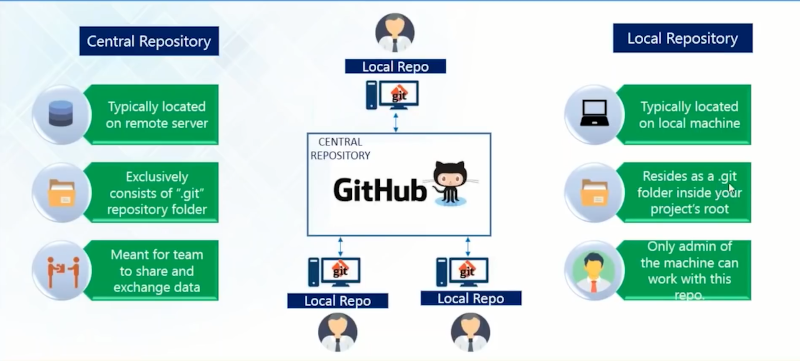
\includegraphics{https://github.com/OxfordIHTM/open-reproducible-science/blob/main/images/git_and_github01b.png}

To use GitHub, you will need create an account at \url{https://github.com}.

\hypertarget{creating-a-github-account}{%
\subsection{Creating a GitHub account}\label{creating-a-github-account}}

\begin{enumerate}
\def\labelenumi{\arabic{enumi}.}
\item
  Head to \url{https://github.com}
\item
  On the upper right hand corner of the page, click on \textbf{Sign-up} button
\end{enumerate}


\includegraphics{images/github_account1.png}

\begin{enumerate}
\def\labelenumi{\arabic{enumi}.}
\setcounter{enumi}{2}
\tightlist
\item
  You will be then prompted to provide an email address to register your account with.
\end{enumerate}

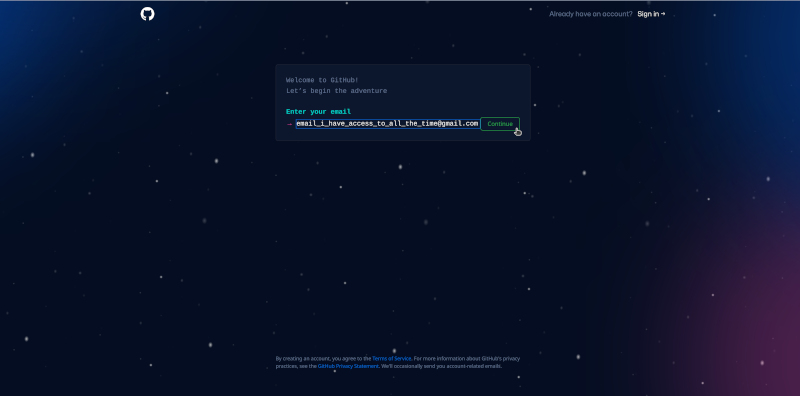
\includegraphics{images/github_account2.png}

With regard to the email address to use for creating a GitHub account, a best practice recommendation is to use an email address that you will have access to all the time. Email addresses such as those for school (if you are a student) or for your current work may not always be the best email address to use as these email addresses tend to be time-limited (i.e., you lose the email address once you graduate or once you leave your current work).

\begin{enumerate}
\def\labelenumi{\arabic{enumi}.}
\setcounter{enumi}{3}
\tightlist
\item
  You will then be prompted for a password.
\end{enumerate}

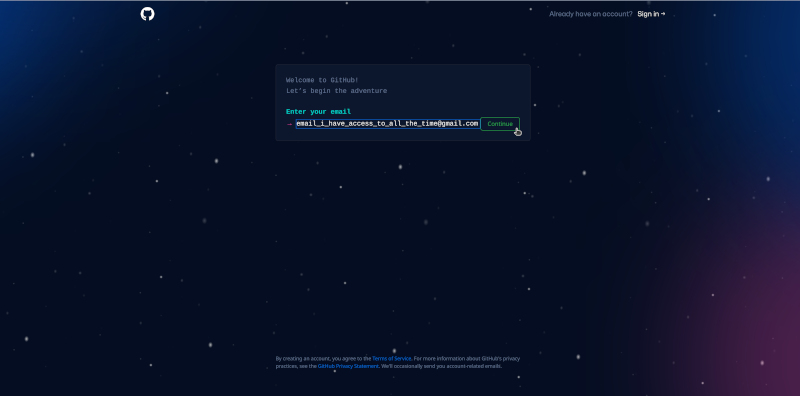
\includegraphics{images/github_account2.png}

\begin{enumerate}
\def\labelenumi{\arabic{enumi}.}
\setcounter{enumi}{4}
\tightlist
\item
  Then follow all other prompts after this including confirmation of your email and creating a GitHub username.
\end{enumerate}

With regard to creating/selecting a GitHub username, following are some best practice recommendations:

\begin{itemize}
\item
  Incorporate your actual name! People like to know who they're dealing with. Also makes your username easier for people to guess or remember.
\item
  Pick a username you will be comfortable revealing to your future boss and/or to future collaborators.
\item
  Shorter is better than longer.
\item
  Be as unique as possible in as few characters as possible. In some settings GitHub auto-completes or suggests usernames.
\item
  Make it timeless. Don't highlight your current university, employer, or place of residence.
\item
  Avoid the use of upper vs.~lower case to separate words. We highly recommend all lowercase. GitHub treats usernames in a case insensitive way, but using all lowercase is kinder to people doing downstream regular expression work with usernames, in various languages. A better strategy for word separation is to use a hyphen \texttt{-}.
\item
  You can change your username later, but better to get this right the first time.
\end{itemize}

\url{https://help.github.com/articles/changing-your-github-username/}

\url{https://help.github.com/articles/what-happens-when-i-change-my-username/}

\begin{enumerate}
\def\labelenumi{\arabic{enumi}.}
\setcounter{enumi}{5}
\tightlist
\item
  Once you have created a GitHub account, please do share your username to the lecture seriese presenter so he can add your username to the Oxford IHTM GitHub account and add you to the Oxford IHTM GitHub Classroom.
\end{enumerate}

\hypertarget{connect-github-rstudio}{%
\chapter{Connecting GitHub with RStudio}\label{connect-github-rstudio}}

\hypertarget{write-functions}{%
\chapter{Writing functions}\label{write-functions}}

For this topic, we will use data on weight and height to calculate body mass index. As a refresher, body mass index is calculated as follows:

\[ \text{Body mass index} ~=~ \frac{weight ~ (kgs)}{height ~ (m) ^ 2} \]
For this topic on writing functions in R, we will use BMI as an example to explore and demonstrate how we can create our own functions in R.

Let's say for example that you have been doing a research on children aged 11 years and older in 3 schools and you have collected the following data:

\textbf{School 1516}

\begin{Shaded}
\begin{Highlighting}[]
\NormalTok{school1516}
\end{Highlighting}
\end{Shaded}

\begin{verbatim}
##     school sex ageMonths weight height
## 427   1516   1       138   24.5  126.0
## 428   1516   1       150   28.3  136.3
## 429   1516   1       162   32.2  143.5
## 430   1516   1       162   32.7  143.5
## 431   1516   1       150   28.6  137.0
## 432   1516   2       138   26.5  134.0
## 433   1516   1       150   29.9  139.2
## 434   1516   1       150   30.0  139.5
## 435   1516   1       162   34.0  148.0
## 436   1516   1       138   25.4  135.7
## 437   1516   1       150   32.3  143.0
## 438   1516   2       174   38.3  153.5
## 439   1516   2       162   41.6  151.0
## 440   1516   1       150   30.7  145.0
## 441   1516   2       186   46.8  155.2
## 442   1516   1       186   46.6  163.4
## 443   1516   1       150   33.5  145.5
## 444   1516   1       186   47.0  164.0
## 445   1516   1       174   41.1  159.5
## 446   1516   2       162   39.1  152.2
## 447   1516   2       174   40.9  155.5
## 448   1516   2       162   39.7  153.0
## 449   1516   2       162   40.9  153.2
## 450   1516   1       150   34.2  147.5
## 451   1516   2       150   41.8  149.4
## 452   1516   1       138   28.0  141.5
## 453   1516   1       138   30.0  142.0
## 454   1516   1       138   33.1  142.0
## 455   1516   1       186   46.1  167.5
## 456   1516   1       150   36.2  149.0
## 457   1516   2       162   47.4  156.0
## 458   1516   1       150   30.3  150.2
## 459   1516   2       150   36.4  152.1
## 460   1516   2       150   36.4  155.0
## 461   1516   2       150   44.1  155.0
## 462   1516   2       162   42.3  160.1
## 463   1516   2       179   50.4  163.5
## 464   1516   1       150   37.6  155.0
## 465   1516   2       138   36.0  154.5
## 466   1516   2       138   46.1  156.0
\end{verbatim}

\textbf{School 1522}

\begin{Shaded}
\begin{Highlighting}[]
\NormalTok{school1522}
\end{Highlighting}
\end{Shaded}

\begin{verbatim}
##     school sex ageMonths weight height
## 646   1522   1       203   30.6  140.5
## 647   1522   1       174   30.8  140.0
## 648   1522   1       162   29.3  136.3
## 649   1522   1       150   24.0  132.0
## 650   1522   1       150   28.1  132.1
## 651   1522   2       150   27.2  134.9
## 652   1522   1       162   34.2  139.2
## 653   1522   1       150   25.5  134.2
## 654   1522   1       138   24.6  129.0
## 655   1522   1       174   36.4  147.5
## 656   1522   1       150   28.7  137.5
## 657   1522   1       186   45.8  155.6
## 658   1522   1       174   36.3  151.6
## 659   1522   1       150   31.0  139.5
## 660   1522   1       138   29.0  134.3
## 661   1522   1       179   38.3  155.5
## 662   1522   2       138   31.3  138.4
## 663   1522   1       162   36.5  148.8
## 664   1522   1       155   36.8  145.2
## 665   1522   1       138   28.3  136.8
## 666   1522   1       138   26.8  137.3
## 667   1522   2       138   32.6  141.4
## 668   1522   2       138   31.9  143.0
## 669   1522   1       174   42.6  160.7
## 670   1522   2       198   57.8  158.0
## 671   1522   2       162   43.9  153.5
## 672   1522   2       150   35.1  150.6
## 673   1522   2       186   52.6  159.6
## 674   1522   2       150   45.1  152.8
## 675   1522   2       138   34.6  147.2
## 676   1522   2       150   45.3  153.1
## 677   1522   1       186   51.8  170.2
## 678   1522   2       150   57.1  154.2
## 679   1522   2       138   33.5  149.2
## 680   1522   1       150   36.3  154.1
## 681   1522   1       174   44.0  169.1
## 682   1522   2       150   44.5  158.3
## 683   1522   2       150   51.5  159.1
## 684   1522   2       138   47.4  157.8
## 685   1522   2       138   36.8  158.5
## 686   1522   2       138   52.0  161.0
\end{verbatim}

\textbf{School 1525}

\begin{Shaded}
\begin{Highlighting}[]
\NormalTok{school1525}
\end{Highlighting}
\end{Shaded}

\begin{verbatim}
##     school sex ageMonths weight height
## 752   1525   1       186   26.2    137
## 753   1525   1       186   32.7    138
## 754   1525   1       150   25.9    130
## 755   1525   1       162   30.4    137
## 756   1525   2       138   24.4    129
## 757   1525   2       138   23.8    130
## 758   1525   1       150   26.1    133
## 759   1525   1       150   26.4    135
## 760   1525   1       174   35.1    148
## 761   1525   1       162   28.7    142
## 762   1525   1       150   28.0    136
## 763   1525   1       174   34.0    149
## 764   1525   1       186   40.6    155
## 765   1525   2       150   35.8    142
## 766   1525   1       150   35.4    140
## 767   1525   2       138   27.8    137
## 768   1525   2       138   28.2    137
## 769   1525   2       138   29.7    139
## 770   1525   2       138   30.9    139
## 771   1525   1       138   28.2    137
## 772   1525   2       138   26.2    140
## 773   1525   2       138   26.6    140
## 774   1525   1       138   27.2    138
## 775   1525   2       138   27.0    141
## 776   1525   1       150   31.3    145
## 777   1525   2       162   33.9    152
## 778   1525   2       162   42.0    153
## 779   1525   2       185   38.3    157
## 780   1525   2       138   31.0    145
## 781   1525   2       138   32.3    145
## 782   1525   1       139   35.1    144
## 783   1525   2       150   36.4    152
## 784   1525   2       138   32.7    147
## 785   1525   1       174   44.9    166
## 786   1525   2       138   32.2    148
## 787   1525   2       138   36.4    148
## 788   1525   1       138   31.4    146
## 789   1525   2       138   45.0    149
## 790   1525   2       162   49.4    160
## 791   1525   2       138   34.3    150
## 792   1525   1       138   30.0    148
## 793   1525   2       150   37.0    156
## 794   1525   2       162   52.2    165
## 795   1525   2       138   42.9    158
\end{verbatim}

In this dataset, the units of the height measurement is in centimetres.

Using what we have learned earlier on calculating BMI using R, I can perform the following R commands to get the BMI for each child in each of the schools:

\begin{Shaded}
\begin{Highlighting}[]
\DocumentationTok{\#\# Calculate BMI for children in school 1516}
\NormalTok{school1516}\SpecialCharTok{$}\NormalTok{weight }\SpecialCharTok{/}\NormalTok{ (school1516}\SpecialCharTok{$}\NormalTok{height }\SpecialCharTok{/} \DecValTok{100}\NormalTok{) }\SpecialCharTok{\^{}} \DecValTok{2}

\DocumentationTok{\#\# Calculate BMI for children in school 1516}
\NormalTok{school1522}\SpecialCharTok{$}\NormalTok{weight }\SpecialCharTok{/}\NormalTok{ (school1516}\SpecialCharTok{$}\NormalTok{height }\SpecialCharTok{/} \DecValTok{100}\NormalTok{) }\SpecialCharTok{\^{}} \DecValTok{2}

\DocumentationTok{\#\# Calculate BMI for children in school 1516}
\NormalTok{school1525}\SpecialCharTok{$}\NormalTok{weight }\SpecialCharTok{/}\NormalTok{ (school1516}\SpecialCharTok{$}\NormalTok{height }\SpecialCharTok{/} \DecValTok{100}\NormalTok{) }\SpecialCharTok{\^{}} \DecValTok{2}
\end{Highlighting}
\end{Shaded}

Because the commands are repetitive, I can easily copy and paste my initial line of code to calculate BMI for children in school 1516 and then just change the object names accordingly to calculate the BMI for children in the two other schools.

When I run these lines of code, I get the following results:

\begin{Shaded}
\begin{Highlighting}[]
\DocumentationTok{\#\# Calculate BMI for children in school 1516}
\NormalTok{school1516}\SpecialCharTok{$}\NormalTok{weight }\SpecialCharTok{/}\NormalTok{ (school1516}\SpecialCharTok{$}\NormalTok{height }\SpecialCharTok{/} \DecValTok{100}\NormalTok{) }\SpecialCharTok{\^{}} \DecValTok{2}
\end{Highlighting}
\end{Shaded}

\begin{verbatim}
##  [1] 15.43210 15.23333 15.63695 15.87976 15.23789 14.75830 15.43095 15.41604 15.52228 13.79349 15.79539 16.25481 18.24481
## [14] 14.60166 19.42954 17.45347 15.82409 17.47472 16.15550 16.87903 16.91463 16.95929 17.42632 15.71962 18.72730 13.98444
## [27] 14.87800 16.41539 16.43128 16.30557 19.47732 13.43083 15.73414 15.15088 18.35588 16.50280 18.85363 15.65036 15.08153
## [40] 18.94313
\end{verbatim}

\begin{Shaded}
\begin{Highlighting}[]
\DocumentationTok{\#\# Calculate BMI for children in school 1516}
\NormalTok{school1522}\SpecialCharTok{$}\NormalTok{weight }\SpecialCharTok{/}\NormalTok{ (school1516}\SpecialCharTok{$}\NormalTok{height }\SpecialCharTok{/} \DecValTok{100}\NormalTok{) }\SpecialCharTok{\^{}} \DecValTok{2}
\end{Highlighting}
\end{Shaded}

\begin{verbatim}
## Warning in school1522$weight/(school1516$height/100)^2: longer object length is not a multiple of shorter object length
\end{verbatim}

\begin{verbatim}
##  [1] 19.27438 16.57903 14.22865 11.65487 14.97150 15.14814 17.65012 13.10363 11.23083 19.76704 14.03492 19.43787 15.92035
## [14] 14.74435 12.03967 14.34481 14.78490 13.57079 14.46527 12.21679 11.08343 13.92627 13.59168 19.58058 25.89564 21.92561
## [27] 17.40726 26.08609 16.07485 15.58488 18.61440 22.96095 24.68185 13.94381 15.10926 17.16604 16.64656 21.43600 19.85735
## [40] 15.12163 32.75384
\end{verbatim}

\begin{Shaded}
\begin{Highlighting}[]
\DocumentationTok{\#\# Calculate BMI for children in school 1516}
\NormalTok{school1525}\SpecialCharTok{$}\NormalTok{weight }\SpecialCharTok{/}\NormalTok{ (school1516}\SpecialCharTok{$}\NormalTok{height }\SpecialCharTok{/} \DecValTok{100}\NormalTok{) }\SpecialCharTok{\^{}} \DecValTok{2}
\end{Highlighting}
\end{Shaded}

\begin{verbatim}
## Warning in school1525$weight/(school1516$height/100)^2: longer object length is not a multiple of shorter object length
\end{verbatim}

\begin{verbatim}
##  [1] 16.50290 17.60176 12.57755 14.76284 13.00016 13.25462 13.46983 13.56612 16.02447 15.58555 13.69260 14.42986 17.80624
## [14] 17.02735 14.69670 10.41216 13.32058 11.04253 12.14611 12.17362 10.83529 11.36315 11.58914 12.41023 14.02307 16.93116
## [27] 20.82920 18.99425 11.04923 14.54889 14.42308 16.13472 14.13479 18.68887 13.40271 14.20099 11.74611 18.73049 20.69522
## [40] 14.09435 18.89645 19.91636 25.34934 20.83308
\end{verbatim}

The calculation for the BMI of children in school 1516 seems to have completed without issues and a vector of BMI results have been produced. However, for school 1522 and school 1525, there is a warning saying:

\begin{Shaded}
\begin{Highlighting}[]
\DocumentationTok{\#\# Warning in school1522$weight/(school1516$height)\^{}2: longer object length is not a multiple}
\DocumentationTok{\#\# of shorter object length}
\end{Highlighting}
\end{Shaded}

Although a result has been provided, the warning gives me an indication that someting is not quite right with my calculation and when I inspect further, I notice that in my formula for school 1522 and for school 1525, my denominator is still using data for school 1516 and this is most likely what is causing the warning message.

So, to correct this I go back to my lines of code and edit the denominators for school 1522 and school 1525 as follows:

\begin{Shaded}
\begin{Highlighting}[]
\DocumentationTok{\#\# Calculate BMI for children in school 1516}
\NormalTok{school1516}\SpecialCharTok{$}\NormalTok{weight }\SpecialCharTok{/}\NormalTok{ (school1516}\SpecialCharTok{$}\NormalTok{height }\SpecialCharTok{/} \DecValTok{100}\NormalTok{) }\SpecialCharTok{\^{}} \DecValTok{2}

\DocumentationTok{\#\# Calculate BMI for children in school 1516}
\NormalTok{school1522}\SpecialCharTok{$}\NormalTok{weight }\SpecialCharTok{/}\NormalTok{ (school1522}\SpecialCharTok{$}\NormalTok{height }\SpecialCharTok{/} \DecValTok{100}\NormalTok{) }\SpecialCharTok{\^{}} \DecValTok{2}

\DocumentationTok{\#\# Calculate BMI for children in school 1516}
\NormalTok{school1525}\SpecialCharTok{$}\NormalTok{weight }\SpecialCharTok{/}\NormalTok{ (school1525}\SpecialCharTok{$}\NormalTok{height }\SpecialCharTok{/} \DecValTok{100}\NormalTok{) }\SpecialCharTok{\^{}} \DecValTok{2}
\end{Highlighting}
\end{Shaded}

which gives me:

\begin{Shaded}
\begin{Highlighting}[]
\DocumentationTok{\#\# Calculate BMI for children in school 1516}
\NormalTok{school1516}\SpecialCharTok{$}\NormalTok{weight }\SpecialCharTok{/}\NormalTok{ (school1516}\SpecialCharTok{$}\NormalTok{height }\SpecialCharTok{/} \DecValTok{100}\NormalTok{) }\SpecialCharTok{\^{}} \DecValTok{2}
\end{Highlighting}
\end{Shaded}

\begin{verbatim}
##  [1] 15.43210 15.23333 15.63695 15.87976 15.23789 14.75830 15.43095 15.41604 15.52228 13.79349 15.79539 16.25481 18.24481
## [14] 14.60166 19.42954 17.45347 15.82409 17.47472 16.15550 16.87903 16.91463 16.95929 17.42632 15.71962 18.72730 13.98444
## [27] 14.87800 16.41539 16.43128 16.30557 19.47732 13.43083 15.73414 15.15088 18.35588 16.50280 18.85363 15.65036 15.08153
## [40] 18.94313
\end{verbatim}

\begin{Shaded}
\begin{Highlighting}[]
\DocumentationTok{\#\# Calculate BMI for children in school 1516}
\NormalTok{school1522}\SpecialCharTok{$}\NormalTok{weight }\SpecialCharTok{/}\NormalTok{ (school1522}\SpecialCharTok{$}\NormalTok{height }\SpecialCharTok{/} \DecValTok{100}\NormalTok{) }\SpecialCharTok{\^{}} \DecValTok{2}
\end{Highlighting}
\end{Shaded}

\begin{verbatim}
##  [1] 15.50132 15.71429 15.77161 13.77410 16.10277 14.94669 17.65012 14.15908 14.78277 16.73082 15.18017 18.91674 15.79459
## [14] 15.92991 16.07852 15.83937 16.34076 16.48493 17.45479 15.12217 14.21653 16.30492 15.59978 16.49597 23.15334 18.63150
## [27] 15.47594 20.65000 19.31656 15.96837 19.32626 17.88178 24.01416 15.04898 15.28626 15.38741 17.75817 20.34543 19.03550
## [40] 14.64837 20.06095
\end{verbatim}

\begin{Shaded}
\begin{Highlighting}[]
\DocumentationTok{\#\# Calculate BMI for children in school 1516}
\NormalTok{school1525}\SpecialCharTok{$}\NormalTok{weight }\SpecialCharTok{/}\NormalTok{ (school1525}\SpecialCharTok{$}\NormalTok{height }\SpecialCharTok{/} \DecValTok{100}\NormalTok{) }\SpecialCharTok{\^{}} \DecValTok{2}
\end{Highlighting}
\end{Shaded}

\begin{verbatim}
##  [1] 13.95919 17.17076 15.32544 16.19692 14.66258 14.08284 14.75493 14.48560 16.02447 14.23329 15.13841 15.31463 16.89906
## [14] 17.75441 18.06122 14.81166 15.02477 15.37188 15.99296 15.02477 13.36735 13.57143 14.28271 13.58081 14.88704 14.67278
## [27] 17.94182 15.53816 14.74435 15.36266 16.92708 15.75485 15.13258 16.29409 14.70051 16.61797 14.73072 20.26936 19.29687
## [40] 15.24444 13.69613 15.20381 19.17355 17.18475
\end{verbatim}

I now do not get the warning message and the expected length of BMI values for each school has now been produced.

From this short example above, we realise how tedious a task it is to type in the code above every time we need to calculate BMI. Also, it becomes even challenging to debug issues with the code because we have to review and edit (as needed) each iteration of the calculation to see where it may have gone wrong (especially when doing a cut and paste approach).

It would be better (and easier) to have a function that calculates and displays the BMI values automatically. Fortunately, \texttt{R} allows us to do just that.

The \texttt{function()} function allows us to create new functions in \texttt{R} with the following generic syntax:

\begin{Shaded}
\begin{Highlighting}[]
\NormalTok{function\_name }\OtherTok{\textless{}{-}} \ControlFlowTok{function}\NormalTok{(argument1, argument2, ...) \{}
  \DocumentationTok{\#\# Your code here}
\NormalTok{\}}
\end{Highlighting}
\end{Shaded}

Using this template/generic syntax, we apply it to create a function called \texttt{calculate\_bmi} as follows:

\begin{Shaded}
\begin{Highlighting}[]
\NormalTok{calculate\_bmi }\OtherTok{\textless{}{-}} \ControlFlowTok{function}\NormalTok{(weight, height) \{}
\NormalTok{  weight }\SpecialCharTok{/}\NormalTok{ height }\SpecialCharTok{\^{}} \DecValTok{2}
\NormalTok{\}}
\end{Highlighting}
\end{Shaded}

We now have a function for calculating and outputing BMI values.

Let us now test it with our 3 sets of data:

\textbf{School 1516}

\begin{Shaded}
\begin{Highlighting}[]
\FunctionTok{calculate\_bmi}\NormalTok{(}
  \AttributeTok{weight =}\NormalTok{ school1516}\SpecialCharTok{$}\NormalTok{weight,}
  \AttributeTok{height =}\NormalTok{ school1516}\SpecialCharTok{$}\NormalTok{height }\SpecialCharTok{/} \DecValTok{100}
\NormalTok{)}
\end{Highlighting}
\end{Shaded}

\begin{verbatim}
##  [1] 15.43210 15.23333 15.63695 15.87976 15.23789 14.75830 15.43095 15.41604 15.52228 13.79349 15.79539 16.25481 18.24481
## [14] 14.60166 19.42954 17.45347 15.82409 17.47472 16.15550 16.87903 16.91463 16.95929 17.42632 15.71962 18.72730 13.98444
## [27] 14.87800 16.41539 16.43128 16.30557 19.47732 13.43083 15.73414 15.15088 18.35588 16.50280 18.85363 15.65036 15.08153
## [40] 18.94313
\end{verbatim}

\textbf{School 1522}

\begin{Shaded}
\begin{Highlighting}[]
\FunctionTok{calculate\_bmi}\NormalTok{(}
  \AttributeTok{weight =}\NormalTok{ school1522}\SpecialCharTok{$}\NormalTok{weight,}
  \AttributeTok{height =}\NormalTok{ school1522}\SpecialCharTok{$}\NormalTok{height }\SpecialCharTok{/} \DecValTok{100}
\NormalTok{)}
\end{Highlighting}
\end{Shaded}

\begin{verbatim}
##  [1] 15.50132 15.71429 15.77161 13.77410 16.10277 14.94669 17.65012 14.15908 14.78277 16.73082 15.18017 18.91674 15.79459
## [14] 15.92991 16.07852 15.83937 16.34076 16.48493 17.45479 15.12217 14.21653 16.30492 15.59978 16.49597 23.15334 18.63150
## [27] 15.47594 20.65000 19.31656 15.96837 19.32626 17.88178 24.01416 15.04898 15.28626 15.38741 17.75817 20.34543 19.03550
## [40] 14.64837 20.06095
\end{verbatim}

\textbf{School 1525}

\begin{Shaded}
\begin{Highlighting}[]
\FunctionTok{calculate\_bmi}\NormalTok{(}
  \AttributeTok{weight =}\NormalTok{ school1525}\SpecialCharTok{$}\NormalTok{weight,}
  \AttributeTok{height =}\NormalTok{ school1525}\SpecialCharTok{$}\NormalTok{height }\SpecialCharTok{/} \DecValTok{100}
\NormalTok{)}
\end{Highlighting}
\end{Shaded}

\begin{verbatim}
##  [1] 13.95919 17.17076 15.32544 16.19692 14.66258 14.08284 14.75493 14.48560 16.02447 14.23329 15.13841 15.31463 16.89906
## [14] 17.75441 18.06122 14.81166 15.02477 15.37188 15.99296 15.02477 13.36735 13.57143 14.28271 13.58081 14.88704 14.67278
## [27] 17.94182 15.53816 14.74435 15.36266 16.92708 15.75485 15.13258 16.29409 14.70051 16.61797 14.73072 20.26936 19.29687
## [40] 15.24444 13.69613 15.20381 19.17355 17.18475
\end{verbatim}

In our example here, the \texttt{calculate\_bmi()} function helped a little bit in making the code to calculate BMI for each student in each school more efficient. But the efficiency that functions provide become more evident when you need to make more complex operations. For example, what if you need to get the mean BMI for students in each school? Without a function, we will have to do the following script for each school:

\textbf{School 1516}

\begin{Shaded}
\begin{Highlighting}[]
\DocumentationTok{\#\# Calculate BMI for children in school 1516}
\NormalTok{bmi\_school1516 }\OtherTok{\textless{}{-}}\NormalTok{ school1516}\SpecialCharTok{$}\NormalTok{weight }\SpecialCharTok{/}\NormalTok{ (school1516}\SpecialCharTok{$}\NormalTok{height }\SpecialCharTok{/} \DecValTok{100}\NormalTok{) }\SpecialCharTok{\^{}} \DecValTok{2}

\DocumentationTok{\#\# Get the mean BMI for children in school 1516}
\NormalTok{mean\_bmi\_school1516 }\OtherTok{\textless{}{-}} \FunctionTok{mean}\NormalTok{(bmi\_school1516)}

\NormalTok{mean\_bmi\_school1516}
\end{Highlighting}
\end{Shaded}

\begin{verbatim}
## [1] 16.28491
\end{verbatim}

\textbf{School 1522}

\begin{Shaded}
\begin{Highlighting}[]
\DocumentationTok{\#\# Calculate BMI for children in school 1522}
\NormalTok{bmi\_school1522 }\OtherTok{\textless{}{-}}\NormalTok{ school1522}\SpecialCharTok{$}\NormalTok{weight }\SpecialCharTok{/}\NormalTok{ (school1522}\SpecialCharTok{$}\NormalTok{height }\SpecialCharTok{/} \DecValTok{100}\NormalTok{) }\SpecialCharTok{\^{}} \DecValTok{2}

\DocumentationTok{\#\# Get the mean BMI for children in school 1522}
\NormalTok{mean\_bmi\_school1522 }\OtherTok{\textless{}{-}} \FunctionTok{mean}\NormalTok{(bmi\_school1522)}

\NormalTok{mean\_bmi\_school1522}
\end{Highlighting}
\end{Shaded}

\begin{verbatim}
## [1] 16.89955
\end{verbatim}

\textbf{School 1525}

\begin{Shaded}
\begin{Highlighting}[]
\DocumentationTok{\#\# Calculate BMI for children in school 1525}
\NormalTok{bmi\_school1525 }\OtherTok{\textless{}{-}}\NormalTok{ school1525}\SpecialCharTok{$}\NormalTok{weight }\SpecialCharTok{/}\NormalTok{ (school1525}\SpecialCharTok{$}\NormalTok{height) }\SpecialCharTok{\^{}} \DecValTok{2}

\DocumentationTok{\#\# Get the mean BMI for children in school 1525}
\NormalTok{mean\_bmi\_school1525 }\OtherTok{\textless{}{-}} \FunctionTok{mean}\NormalTok{(bmi\_school1525)}

\NormalTok{mean\_bmi\_school1525}
\end{Highlighting}
\end{Shaded}

\begin{verbatim}
## [1] 0.001564695
\end{verbatim}

As the operations/calculations we want to perform become more complex, the copy and paste method becomes more and more tedious. With the function approach, we can use the following:

\begin{Shaded}
\begin{Highlighting}[]
\NormalTok{calculate\_mean\_bmi }\OtherTok{\textless{}{-}} \ControlFlowTok{function}\NormalTok{(weight, height) \{}
\NormalTok{  bmi }\OtherTok{\textless{}{-}}\NormalTok{ weight }\SpecialCharTok{/}\NormalTok{ height }\SpecialCharTok{\^{}} \DecValTok{2}
  
\NormalTok{  mean\_bmi }\OtherTok{\textless{}{-}} \FunctionTok{mean}\NormalTok{(bmi)}
  
  \FunctionTok{return}\NormalTok{(mean\_bmi)}
\NormalTok{\}}
\end{Highlighting}
\end{Shaded}

Applying the function to the datasets, we get:

\textbf{School 1516}

\begin{Shaded}
\begin{Highlighting}[]
\FunctionTok{calculate\_mean\_bmi}\NormalTok{(}
  \AttributeTok{weight =}\NormalTok{ school1516}\SpecialCharTok{$}\NormalTok{weight,}
  \AttributeTok{height =}\NormalTok{ school1516}\SpecialCharTok{$}\NormalTok{height }\SpecialCharTok{/} \DecValTok{100}
\NormalTok{)}
\end{Highlighting}
\end{Shaded}

\begin{verbatim}
## [1] 16.28491
\end{verbatim}

\textbf{School 1522}

\begin{Shaded}
\begin{Highlighting}[]
\FunctionTok{calculate\_mean\_bmi}\NormalTok{(}
  \AttributeTok{weight =}\NormalTok{ school1522}\SpecialCharTok{$}\NormalTok{weight,}
  \AttributeTok{height =}\NormalTok{ school1522}\SpecialCharTok{$}\NormalTok{height }\SpecialCharTok{/} \DecValTok{100}
\NormalTok{)}
\end{Highlighting}
\end{Shaded}

\begin{verbatim}
## [1] 16.89955
\end{verbatim}

\textbf{School 1525}

\begin{Shaded}
\begin{Highlighting}[]
\FunctionTok{calculate\_mean\_bmi}\NormalTok{(}
  \AttributeTok{weight =}\NormalTok{ school1525}\SpecialCharTok{$}\NormalTok{weight,}
  \AttributeTok{height =}\NormalTok{ school1525}\SpecialCharTok{$}\NormalTok{height }\SpecialCharTok{/} \DecValTok{100}
\NormalTok{)}
\end{Highlighting}
\end{Shaded}

\begin{verbatim}
## [1] 15.64695
\end{verbatim}

\hypertarget{clone-repository}{%
\chapter{Cloning a GitHub repository into your local computer using RStudio}\label{clone-repository}}

This tutorial is a summary of the the instructions described here - \url{https://docs.github.com/en/repositories/creating-and-managing-repositories/cloning-a-repository}.

\hypertarget{copy-the-repository-url-of-the-repository-you-want-to-clone-from-github}{%
\section{Copy the repository URL of the repository you want to clone from GitHub}\label{copy-the-repository-url-of-the-repository-you-want-to-clone-from-github}}

\includegraphics{https://user-images.githubusercontent.com/5742010/152893606-447d3b63-b5a4-4191-8e2e-5457d2431354.png}

7.1.1 Go to the GitHub page of the repository you own and click on the green button that is labeled code

7.1.2 Click on the copy to clipboard icon to copy the repository URL.

\hypertarget{go-to-rstudio-and-create-new-project}{%
\section{Go to RStudio and create new project}\label{go-to-rstudio-and-create-new-project}}

\includegraphics{https://user-images.githubusercontent.com/5742010/152893999-12eb6fb5-f37f-45e2-99bb-ab752c8d28b2.png}

\hypertarget{choose-version-control}{%
\section{Choose Version Control}\label{choose-version-control}}

\includegraphics{https://user-images.githubusercontent.com/5742010/152894141-d70d33b1-23cc-433d-a06e-0f6eb90a5521.png}

\hypertarget{select-git}{%
\section{Select Git}\label{select-git}}

\includegraphics{https://user-images.githubusercontent.com/5742010/152894209-da871ce4-830b-4e7f-9ca5-7610447bfef4.png}

\hypertarget{setup-repository-settings}{%
\section{Setup repository settings}\label{setup-repository-settings}}

\includegraphics{https://user-images.githubusercontent.com/5742010/152894284-58d28f50-97db-44ec-8363-152f90286610.png}

7.5.1 Paste the repository URL you copied earlier.

7.5.2 The Project directory name should be specified already after you paste the repository URL. Use the suggested directory name.

7.5.3 Browse for the directory on your local computer where you want to save the files for the specified project.

7.5.4 Click on the \texttt{Create\ Project} button/icon.

You will now have the GitHub repository in your local computer.

\hypertarget{commit-and-push}{%
\chapter{Committing your changes and pushing them to GitHub}\label{commit-and-push}}

Following are the steps to take in committing your changes in RStudio and pushing them to GitHub.

\hypertarget{click-on-commit-in-the-git-tab-on-rstudio}{%
\section{\texorpdfstring{Click on \texttt{Commit} in the Git tab on RStudio}{Click on Commit in the Git tab on RStudio}}\label{click-on-commit-in-the-git-tab-on-rstudio}}

\includegraphics{https://user-images.githubusercontent.com/5742010/152895564-b9fb8960-89da-4b86-8d42-c9687d60fad4.png}

\hypertarget{getting-changes-saved-and-push-to-github}{%
\section{Getting changes saved and push to GitHub}\label{getting-changes-saved-and-push-to-github}}

\includegraphics{https://user-images.githubusercontent.com/5742010/152895737-33181b80-c484-444a-bda8-19ee027970d0.png}

8.2.1 Tick the box beside the file that has changed to stage the changes.

8.2.2 Write a commit message in the \texttt{Commit\ message} dialog box. In the commit message, describe the changes that you made.

8.2.3 Click on the \texttt{Commit} button.

8.2.4 Click on the \texttt{Push} button.

\hypertarget{portable-reproducible}{%
\chapter{Creating portable and reproducible scientific workflows}\label{portable-reproducible}}

At this point, you would have written your own R code and R scripts and saved these within an R file (\texttt{.R}).

By now, you would have also appreciated how extensible R is through built-in packages and/or through functions that you have created yourself.

So far, in the examples that we have worked on, the operations and the problems have been quite straightforward. But from your own experience dealing with your own data, real world data is far from straightforward and far from simple. Complexity is almost always a given.

R's scripting capability and R's extensibility are its main characteristics that make R a good tool for creating robust scientific workflows particularly for complex data and research projects.

A typical scientific workflow would have the following steps:

\begin{center}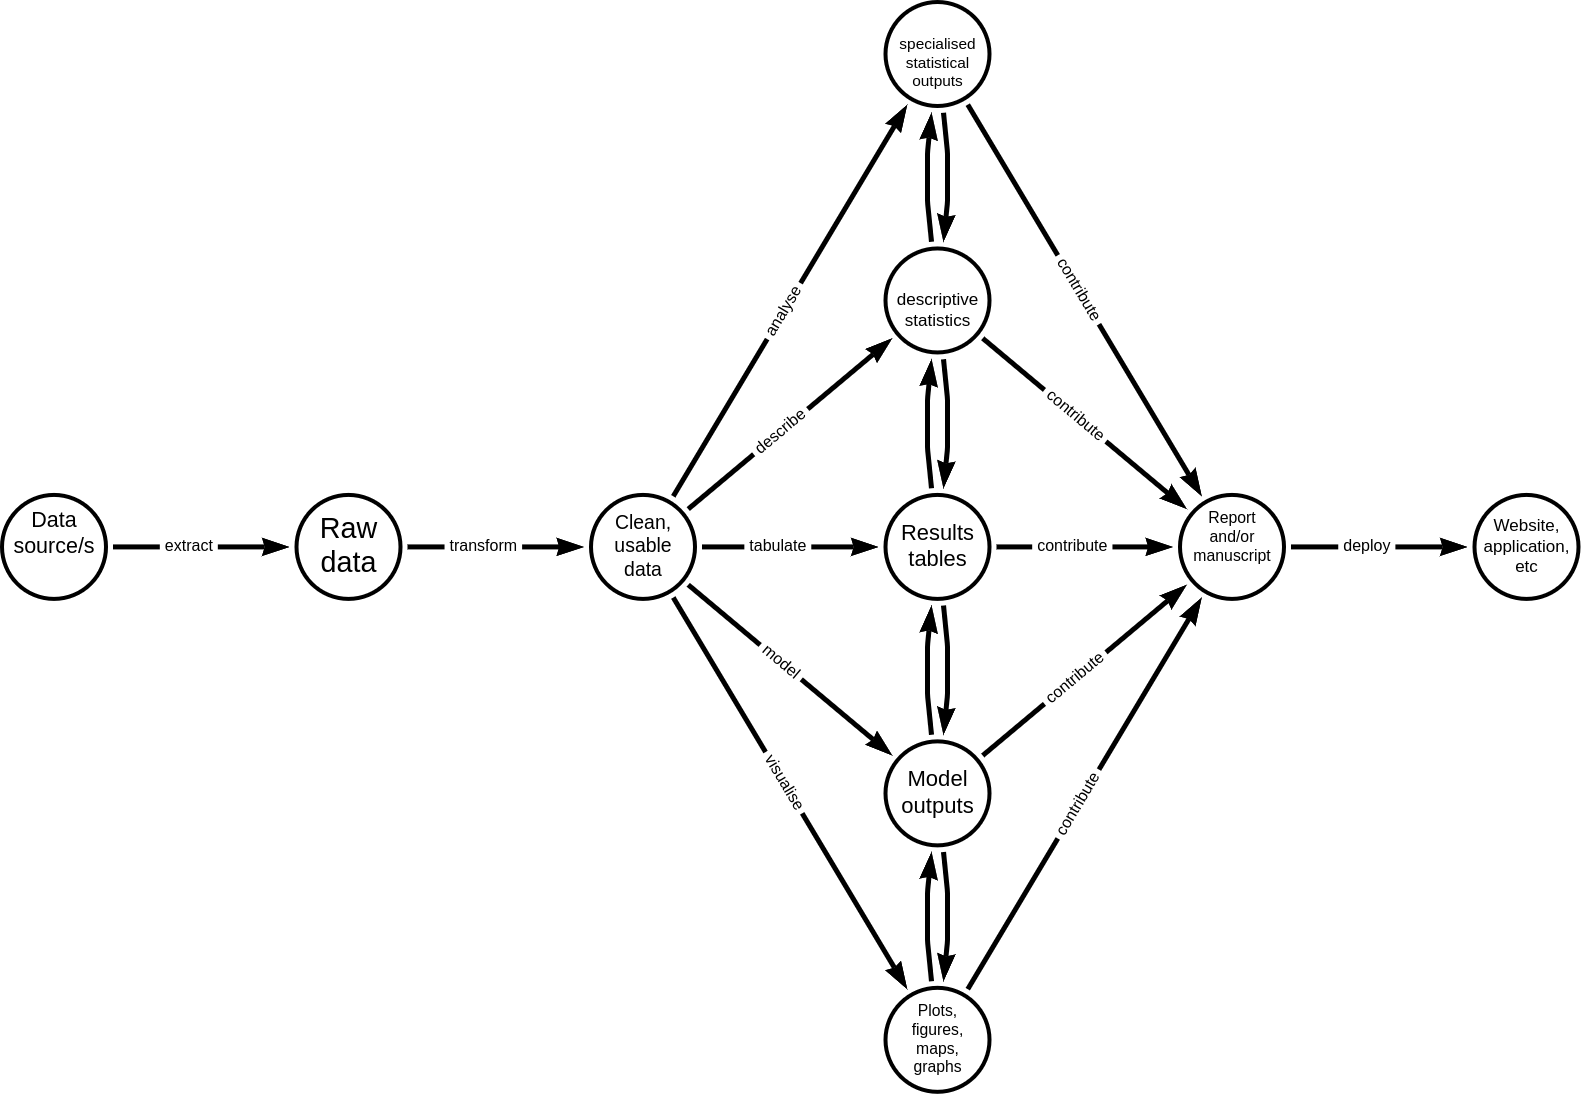
\includegraphics[width=21.96in]{images/scientific-workflow} \end{center}

In general, an R script should reflect the different steps outlined above. Hence, an R script of a scientific workflow would tend to look like this:

\begin{Shaded}
\begin{Highlighting}[]
\DocumentationTok{\#\# Load libraries}


\DocumentationTok{\#\# Retrieve and read data}


\DocumentationTok{\#\# Process data}


\DocumentationTok{\#\# Analyse data}

\DocumentationTok{\#\#\# Descriptive analysis}

\DocumentationTok{\#\#\# Statistical tests}

\DocumentationTok{\#\#\# Model specifications}


\DocumentationTok{\#\# Outputs}

\DocumentationTok{\#\#\# Tabulation of results}

\DocumentationTok{\#\#\# Model outputs}

\DocumentationTok{\#\#\# Plots}


\DocumentationTok{\#\# Report}

\end{Highlighting}
\end{Shaded}

In this chapter, we will go through a step-by-step walkthrough of how to build a robust scientific workflow in R. A robust worklow is one that is \textbf{portable} i.e., not dependent on hardware and software and instead can be run on almost any machine with very minimal, if any, additional setup or configuration required, and one that is \textbf{reproducible} i.e., can be run over and over again without issues, providing the expected results with the same data or providing updated results with new and/or updated data.

\hypertarget{step-1-create-a-new-rstudio-project}{%
\section{Step 1: Create a new RStudio project}\label{step-1-create-a-new-rstudio-project}}

\begin{itemize}
\item
  Open RStudio
\item
  Click on the \texttt{File} option in the RStudio menu. In the dropdown menu, select \texttt{New\ Project}
\item
  In the menu window, select \texttt{New\ directory} option.
\item
  In the next menu window, select \texttt{New\ project} option.
\item
  In the next menu window, enter the following details:

  \begin{itemize}
  \item
    Name of the project - important to make the project name as short as possible but descriptive of the project you are creating; don't use spaces, instead use dash (or underscore) and avoid using capital letters;
  \item
    Select the directory in your computer in which you want to save the project in. Click on \texttt{Browse} to open your computers file manager and navigate to the directory you want to save your project in;
  \item
    Tick the selection box to make this project a git repository (whilst this is not necessary, this is highly recommended especially if you are collaborating with others);
  \item
    Tick the selection box to enable \texttt{renv} in this project (this is what mainly contribute to the portability of your project); and,
  \item
    Click on \texttt{Create\ project}
  \end{itemize}
\end{itemize}

\hypertarget{step-2-create-an-r-file-called-packages.r}{%
\section{\texorpdfstring{Step 2: Create an R file called \texttt{packages.R}}{Step 2: Create an R file called packages.R}}\label{step-2-create-an-r-file-called-packages.r}}

\begin{itemize}
\item
  Click on the \texttt{File} option in the RStudio menu. In the dropdown menu, select \texttt{New\ File} and then in the next dropdown menu, select \texttt{R\ script}.
\item
  A new tab will open in your text editor pane of RStudio (upper left pane) with the name \emph{Untitled1}. Save this file by clicking on the disk icon on the text editor menu or do a keyboard shortcut with \texttt{CTRL\ +\ s}. Give this empty R script the filename \texttt{packages.R}.
\item
  You should now see a file in the main directory/root directory of your project named \texttt{packages.R}
\item
  Add code in the \texttt{packages.R} file specifying the packages you will be using in this project. There will be standard packages that we will always use with this type of workflow. So a template/generic \texttt{packages.R} file will contain the following:
\end{itemize}

\begin{Shaded}
\begin{Highlighting}[]
\DocumentationTok{\#\#\#\#\#\#\#\#\#\#\#\#\#\#\#\#\#\#\#\#\#\#\#\#\#\#\#\#\#\#\#\#\#\#\#\#\#\#\#\#\#\#\#\#\#\#\#\#\#\#\#\#\#\#\#\#\#\#\#\#\#\#\#\#\#\#\#\#\#\#\#\#\#\#\#\#\#\#\#\#}
\CommentTok{\#}
\CommentTok{\#\textquotesingle{}}
\CommentTok{\#\textquotesingle{} General packages needed for a targets workflow}
\CommentTok{\#\textquotesingle{}}
\CommentTok{\#}
\DocumentationTok{\#\#\#\#\#\#\#\#\#\#\#\#\#\#\#\#\#\#\#\#\#\#\#\#\#\#\#\#\#\#\#\#\#\#\#\#\#\#\#\#\#\#\#\#\#\#\#\#\#\#\#\#\#\#\#\#\#\#\#\#\#\#\#\#\#\#\#\#\#\#\#\#\#\#\#\#\#\#\#\#}

\FunctionTok{library}\NormalTok{(targets)}
\FunctionTok{library}\NormalTok{(tarchetypes)}
\FunctionTok{library}\NormalTok{(here)}
\FunctionTok{library}\NormalTok{(rmarkdown)}
\FunctionTok{library}\NormalTok{(knitr)}
\FunctionTok{library}\NormalTok{(kableExtra)}
\FunctionTok{library}\NormalTok{(dplyr)}
\FunctionTok{library}\NormalTok{(openxlsx)}
\FunctionTok{library}\NormalTok{(ggplot2)}


\DocumentationTok{\#\#\#\#\#\#\#\#\#\#\#\#\#\#\#\#\#\#\#\#\#\#\#\#\#\#\#\#\#\#\#\#\#\#\#\#\#\#\#\#\#\#\#\#\#\#\#\#\#\#\#\#\#\#\#\#\#\#\#\#\#\#\#\#\#\#\#\#\#\#\#\#\#\#\#\#\#\#\#\#}
\CommentTok{\#}
\CommentTok{\#\textquotesingle{}}
\CommentTok{\#\textquotesingle{} Add other packages that will be used in the project below}
\CommentTok{\#\textquotesingle{}}
\CommentTok{\#}
\DocumentationTok{\#\#\#\#\#\#\#\#\#\#\#\#\#\#\#\#\#\#\#\#\#\#\#\#\#\#\#\#\#\#\#\#\#\#\#\#\#\#\#\#\#\#\#\#\#\#\#\#\#\#\#\#\#\#\#\#\#\#\#\#\#\#\#\#\#\#\#\#\#\#\#\#\#\#\#\#\#\#\#\#}


\end{Highlighting}
\end{Shaded}

\hypertarget{step-3-create-placeholder-directories-for-different-components-of-workflow}{%
\section{Step 3: Create placeholder directories for different components of workflow}\label{step-3-create-placeholder-directories-for-different-components-of-workflow}}

\begin{itemize}
\item
  In the lower right pane of RStudio (the file manager pane), find the menu button labelled \texttt{Folder}.
\item
  Give this new folder the label of \texttt{R}. This filder will hold all bespoke functions that we will create to use for this project workflow;
\item
  Repeat these steps to create new folders with the following labels:

  \begin{itemize}
  \item
    \texttt{data} - This folder will hold any data that we retrieve as part of this workflow.
  \item
    \texttt{outputs} - This folder will hold all our workflow outputs such as plots/figures, tables (in Excel or CSV files), HTML and/or Word and/or PDF outputs
  \item
    \texttt{reports} - This folder will hold all our RMarkdown report (\texttt{.Rmd}) files
  \item
    \texttt{docs} - This folder will hold any of our deployed outputs such as HTML report, dashboard, etc.
  \end{itemize}
\end{itemize}

These are placeholder directories which we will populate as we work through the workflow for this project.

\hypertarget{step-4-create-the-target-script-file-_targets.r}{%
\section{\texorpdfstring{Step 4: Create the target script file (\texttt{\_targets.R})}{Step 4: Create the target script file (\_targets.R)}}\label{step-4-create-the-target-script-file-_targets.r}}

The next task is to create a \{targets\} script file (\texttt{\_targets.R}) which is the file that will define the workflow that we will be creating.

Create the file by:

\begin{itemize}
\item
  Clicking on File --\textgreater{} New File --\textgreater{} R Script in RStudio.
\item
  A new tab will show in your Source window on the top left quadrant of your RStudio screen. This tab will usually be called \texttt{Untitled1}.
\item
  Save this file first and change its name to \texttt{\_targets.R}. Make sure to save it in the current project directory.
\item
  You know that you were successful in doing this once you see a file called \texttt{\_targets.R} in the File system window in the lower right quadrant of your RStudio screen.
\end{itemize}

\hypertarget{step-5-edit-the-_targets.r-script-file}{%
\section{\texorpdfstring{Step 5: Edit the \texttt{\_targets.R} script file}{Step 5: Edit the \_targets.R script file}}\label{step-5-edit-the-_targets.r-script-file}}

Now, the next step is to edit your script file by adding sets of R code that does the following:

\begin{itemize}
\tightlist
\item
  Loads the packages required
\item
  Loads custom functions (if any)
\item
  Defines individual targets using \texttt{tar\_targets} function
\item
  Ends with a list of targets objects
\end{itemize}

A basic \texttt{\{targets\}} workflow will look like this:

\begin{Shaded}
\begin{Highlighting}[]
\DocumentationTok{\#\# Load libraries {-}{-}{-}{-}{-}{-}{-}{-}{-}{-}{-}{-}{-}{-}{-}{-}{-}{-}{-}{-}{-}{-}{-}{-}{-}{-}{-}{-}{-}{-}{-}{-}{-}{-}{-}{-}{-}{-}{-}{-}{-}{-}{-}{-}{-}{-}{-}{-}{-}{-}{-}{-}{-}{-}{-}{-}{-}{-}{-}{-}{-}{-}}
\FunctionTok{library}\NormalTok{(targets)}



\DocumentationTok{\#\# Load custom functions {-}{-}{-}{-}{-}{-}{-}{-}{-}{-}{-}{-}{-}{-}{-}{-}{-}{-}{-}{-}{-}{-}{-}{-}{-}{-}{-}{-}{-}{-}{-}{-}{-}{-}{-}{-}{-}{-}{-}{-}{-}{-}{-}{-}{-}{-}{-}{-}{-}{-}{-}{-}{-}{-}{-}}
\ControlFlowTok{for}\NormalTok{ (f }\ControlFlowTok{in} \FunctionTok{list.files}\NormalTok{(}\StringTok{"R"}\NormalTok{, }\AttributeTok{full.names =} \ConstantTok{TRUE}\NormalTok{)) }\FunctionTok{source}\NormalTok{ (f)}
\ControlFlowTok{for}\NormalTok{ (f }\ControlFlowTok{in} \FunctionTok{list.files}\NormalTok{(here}\SpecialCharTok{::}\FunctionTok{here}\NormalTok{(}\StringTok{"R"}\NormalTok{), }\AttributeTok{full.names =} \ConstantTok{TRUE}\NormalTok{)) }\FunctionTok{source}\NormalTok{ (f)}


\DocumentationTok{\#\# Create targets and list targets objects {-}{-}{-}{-}{-}{-}{-}{-}{-}{-}{-}{-}{-}{-}{-}{-}{-}{-}{-}{-}{-}{-}{-}{-}{-}{-}{-}{-}{-}{-}{-}{-}{-}{-}{-}{-}{-}}


\end{Highlighting}
\end{Shaded}


  \bibliography{book.bib}

\end{document}
